\documentclass[a4paper,11pt]{article}
\usepackage{indentfirst}
\usepackage[T1]{fontenc}
\usepackage[polish]{babel}
\usepackage[utf8]{inputenc}
\usepackage{lmodern}
\selectlanguage{polish}
\usepackage[top=2cm, bottom=2cm, left=1cm, right=1cm]{geometry}
\usepackage{lastpage}
\usepackage{fancyhdr}
\pagestyle{fancy}
\setlength\parindent{24pt}
\makeatletter
\newcommand{\linia}{\rule{\linewidth}{0.4mm}}
\renewcommand{\maketitle}{\begin{titlepage}
    \vspace*{2cm}
    \begin{center}\LARGE
    Politechnika Warszawska\\
    Wydział Elektryczny\\
    \end{center}
    \vspace{5cm}
    \noindent\linia
    \begin{center}
      \LARGE \textsc{\@title}
         \end{center}
     \linia
    \vspace{0.5cm}
    \begin{flushright}
    \begin{minipage}{5cm}
    \textit{Autor:}\\
    \normalsize \textsc{\@author} \par
    \end{minipage}
    \vspace{5cm}
     \end{flushright}
    \vspace*{\stretch{6}}
    \begin{center}
    \@date
    \end{center}
  \end{titlepage}
}
\makeatother
\author{Grzegorz Kopyt\\Arkadiusz Michalak}
\title{Sprawozdanie}
\usepackage{graphicx}

\fancyhf{}
\fancyhead[CO,CE]{ Grzegorz Kopyt Arkadiusz Michalak \\ Projekt grupowy - Sprawozdanie Końcowe \\ \today }

\rfoot{\thepage{}/\pageref{LastPage}}

\begin{document}
\maketitle

\tableofcontents
\vspace{1cm}
\noindent\linia
\section{Cel powstania dokumentu}

\noindent\linia
\section{Opis problemu}

\noindent\linia
\section{Wysoko abstrakcyjny opis działania algorytmu}

\noindent\linia
\section{Efekty działania programu}
W czasie trwanie projektu udało się zrealizować wszystkie wymagane funkcjonalności. Najlepszą prezentacją tego jak działa program jest jego uruchomienie. Jednak krótki opis stworzonego interfejsu użytkownika oraz efektów jego działania przedstawiamy poniżej:
\begin{figure}
    \centering
    \caption{Okno główne programu}
    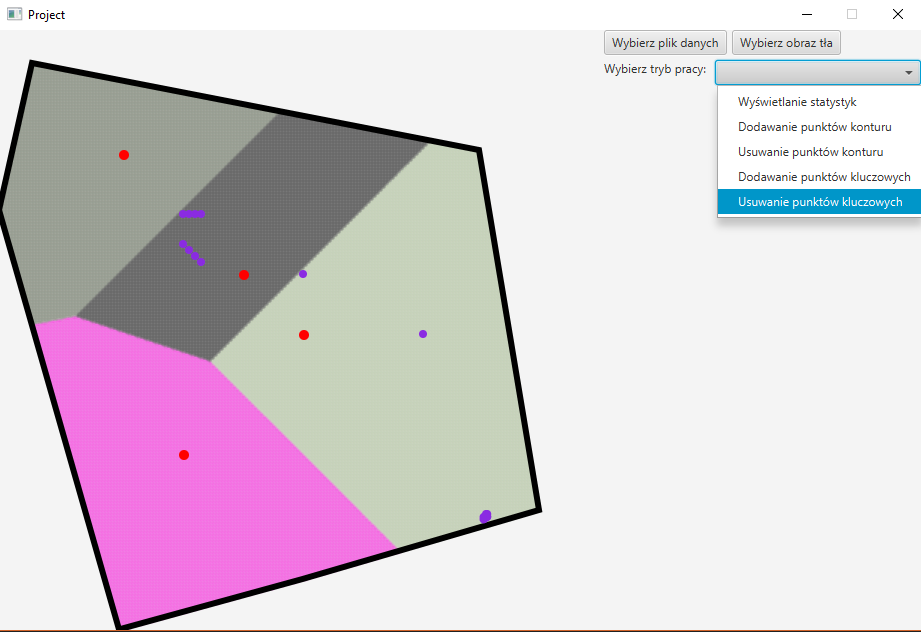
\includegraphics[scale=0.77]{GUI.png}
\end{figure}

\noindent\linia
\section{Zmiany względem specyfikacji}

\noindent\linia
\section{Zmagania z wyznaczaniem optymalnych obszarów}
Szukając sposobu na sprostanie wyzwaniu wyznaczania optymalnych obszarów powstały trzy ścieżki:
\begin{enumerate}
\item Algorytm autorski,
\item Algorytm Fortune'a,
\item Algorytm ostateczny.
\end{enumerate}
\noindent\linia
\section{Podsumowanie i wnioski}

\noindent\linia
\section{Ocena prowadzenia zajęć}

\noindent\linia

\end{document}



